\chapter{Requirement Analysis}
\label{chap:requirement-analysis}

\section{Stakeholder Analysis}
\label{section:stakeholder-analysis}

\begin{itemize}
    \item\textbf{Thai Stock Investors} - The primary stakeholders of VIIV who use online tools and technical resources to analyze stocks and market trends, aiming to maximize investment returns while managing risks. However, the large volume of market data and financial reports can be overwhelming, leading to missed opportunities or emotionally driven investment decisions. 
    \item \textbf{Thai Financial Analysts} - Professionals who evaluate stocks and provide recommendations. VIIV provides AI-powered insights that can complement their research.
\end{itemize}

\section{User Stories}
\label{section:user-stories}

\begin{itemize}
    \item \textbf{Thai Stock Investor:}  
    \begin{itemize}
        \item As a Thai stock investor, I want to receive AI-generated stock analysis in Thai so that I can make informed investment decisions efficiently.
        \item As a Thai stock investor, I want VIIV to summarize 56-1 One Reports and financial statements so that I can quickly understand a company’s financial health without reading lengthy documents.
        \item As a Thai stock investor, I want VIIV to analyze stock price trends using technical indicators such as MACD so that I can determine whether a stock is in an uptrend or downtrend.
        \item As a Thai stock investor, I want VIIV to provide IAA consensus sentiment analysis so that I can assess investment opportunities based on professional analysts' opinions.
        \item As a Thai stock investor, I want VIIV to reduce information overload by filtering relevant stock data so that I can focus on critical insights for decision-making.
        \item As a Thai stock investor, I want VIIV to help minimize my investment risks by identifying potential opportunities and warning signs based on fundamental and technical analysis.
    \end{itemize}

    \item \textbf{Thai Financial Analyst:}  
    \begin{itemize}
        \item As a Thai financial analyst, I want to use VIIV to analyze financial statements and business models so that I can validate investment opportunities efficiently.
        \item As a Thai financial analyst, I want VIIV to generate technical indicators and stock price trend analysis using data-driven methods so that I can enhance my market predictions.
        \item As a Thai financial analyst, I want VIIV to integrate real-time stock data from reliable sources so that I can access up-to-date information when making investment decisions.
        \item As a Thai financial analyst, I want VIIV to automate parts of stock research by extracting key insights from reports and trends so that I can focus on high-level investment strategies.
    \end{itemize}
\end{itemize}



\section{Use Case Diagram}
\label{section:use-case-diagram}
<TIP: Write a use case diagram for your project here. Refer to an
article “What is a use case diagram?” by Lucidchart for help./>

\section{Use Case Model}
\label{section:use-case-model}
A use case is a detailed description of how a system
interacts with an external entity (such as a user or another system) to
accomplish a specific goal. Use cases provide a high-level view of the
functionality of a system and help in capturing and documenting its
requirements from the perspective of end users.

<TIP: Write use cases for your project here. Make sure to use the
appropriate type of use case for each scenario (brief, casual, and fully-dressed
use case)./>

\section{User Interface Design}
\label{section:user-interface-design}

\begin{figure}[h]
    \centering
    \frame{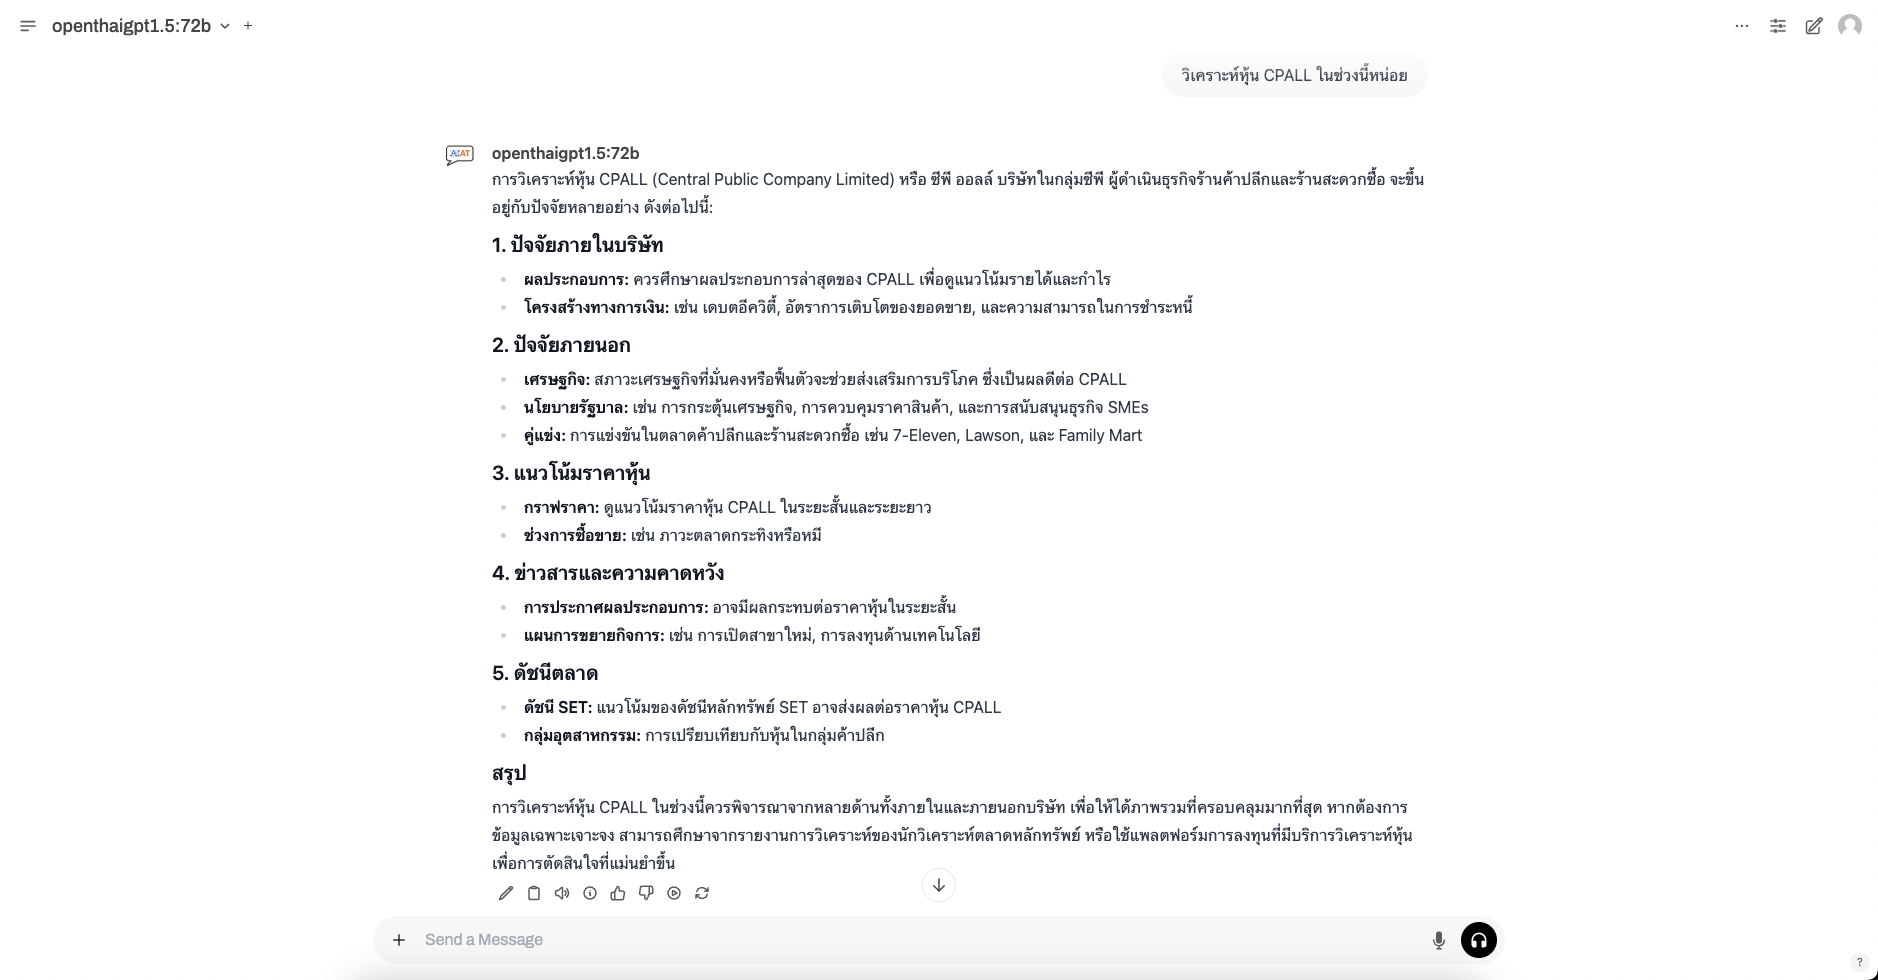
\includegraphics[width=1\textwidth]{chapter-3/viiv-mockup-ui-chat.png}}
    \caption[Mockup UI of VIIV's stock analysis feature]{Mockup UI of VIIV's stock analysis feature. Created by the author, accessed 21 March 2025.}
    \label{fig:viiv-mockup-ui-chat}
\end{figure}

Figure \ref{fig:viiv-mockup-ui-chat} illustrates how the chatbot generates 
a structured response with detailed insights when a user enters a prompt 
about stock analysis. In this example, the user requests an analysis of CPALL stock, 
and the chatbot responds by breaking down the information into key sections. 
The response includes internal company factors, such as profitability and expansion plans, 
external influences, like economic conditions and government policies, stock price trends, 
market news, and market indices that impact CPALL’s performance.

\begin{figure}[h]
    \centering
    \frame{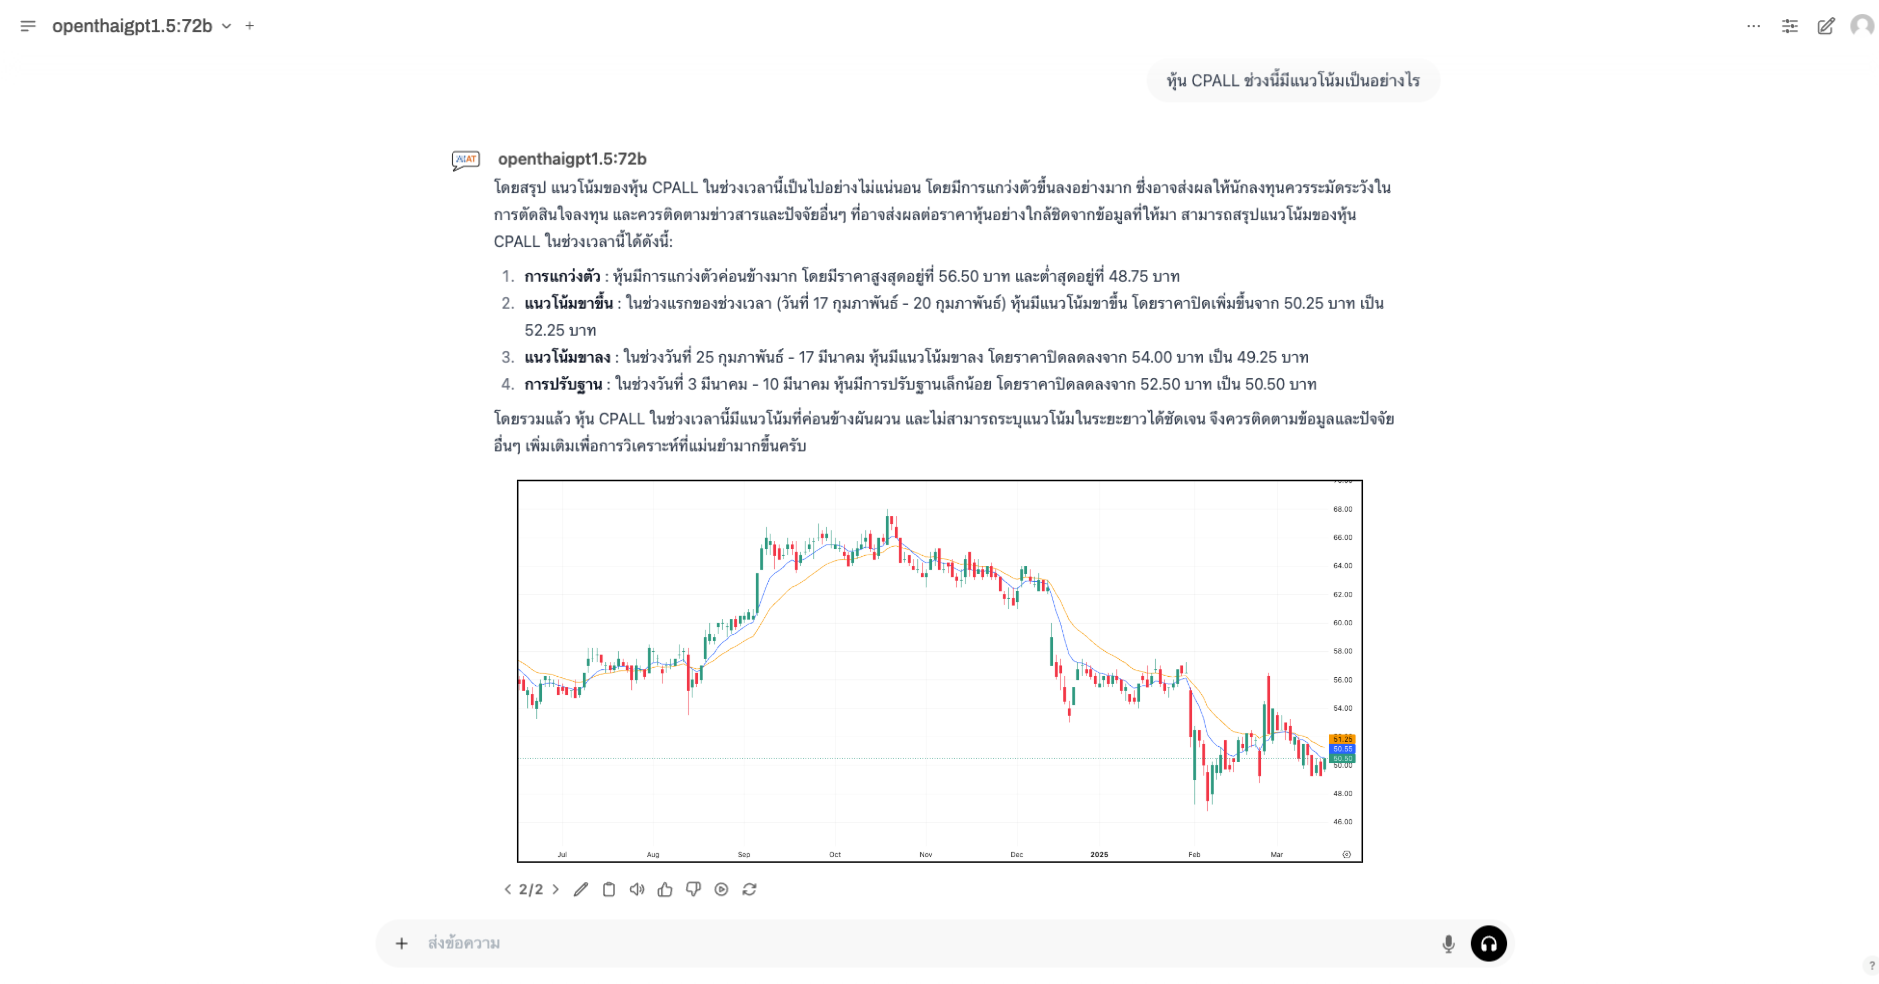
\includegraphics[width=1\textwidth]{chapter-3/viiv-mockup-ui-visualization.png}}
    \caption[Mockup UI of VIIV's stock trend visualization feature]{Mockup UI of VIIV's stock trend visualization feature. Created by the author, accessed 21 March 2025.}
    \label{fig:viiv-mockup-ui-visualization}
\end{figure}

Figure \ref{fig:viiv-mockup-ui-visualization} illustrates the chatbot’s response when
a user asks about the stock trend of CPALL. The chatbot provides a detailed analysis, 
summarizing the stock’s movement over different time periods. It breaks down the stock 
trend into key insights, including price range, upward trend, downward trend, 
and consolidation phase. The response highlights the highest and lowest stock prices, 
periods of increase and decline, and possible market corrections.

Additionally, the UI includes a stock price chart at the bottom, which visually 
represents CPALL’s historical price movements using a candlestick chart and moving averages. 
The chart provides investors with a graphical interpretation of price fluctuations over time.